\chapter{Аналитический раздел}

\section{Описание предметной области}

\section{Метод на основе трассировке лучей}

Метод расчета радиоционно-газодинамических моделей на основе трассировке лучей является точным методом. Идея метода состоит в том, что с площадки испускается семейство лучей. Начальные лучи изображены на рисунке~\ref{fig:rays-start}. 

\begin{figure}[H]
	\centering
	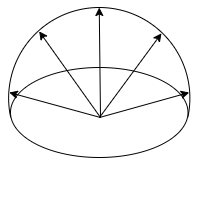
\includegraphics[width=0.5\linewidth]{img/raysStart}
	\caption{}
	\label{fig:rays-start}
\end{figure}

Каждый луч характеризуется направлением $\vec{r}$, начальной точкой $\vec{r_0}$ и интенсивностью $I$. Точка принадлежащая лучу рассчитывается по формуле~(\ref{eq:ray})
\begin{equation}
   \label{eq:ray} 
   \vec{R}(t) = \vec{r_0} + \vec{r} \cdot t
\end{equation}

Каждый луч отслеживается до момента пока не выйдет из системы, поглотится в атмосфере или рассеется. На своем пути луч может отражаться от поверхностей и преломляться, в следствии чего порождать новые лучи. Пример пути луча показан на рисунке~\ref{fig:rays}.

\begin{figure}[H]
    \centering
    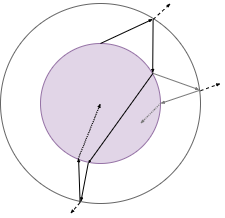
\includegraphics[width=0.5\linewidth]{img/rays}
    \caption{Путь луча}
    \label{fig:rays}
\end{figure}

Отражение луча рассчитывается по формуле~\ref{eq:reflect}.

\begin{equation}
\label{eq:reflect}
    \vec{R} = 2 \vec{n} (\vec{n}\cdot\vec{L}) - \vec{L}
\end{equation}

Преломление луча рассчитывается по формуле~(\ref{eq:refract}).
\begin{equation}
    \label{eq:refract}
    \vec{R} = n \vec{N} (\vec{N} \cdot \vec{L}) - n \vec{L} - \vec{N} \sqrt{1 + n^2((\vec{N} \cdot \vec{L}) - 1)}
\end{equation}

TODO: вставить картинки

\section{Метод дискретных ординат}

Метод дискретных ординат~(МДО)~[\cite{mdo}] считается самым быстрым численным методом теории переноса излучения. МДО применим как для рассеянного солнечного, так и для теплового излучения. Более того, пожалуй, это единственный метод, эффективно работающий сразу для суммы указанных компонент излучения. В рамках МДО можно учесть все особенности отражения от поверхности. Он применим не только для изотропного, но практически для любого типа отражения.  

В основе МДО лежит рассмотрение исходного дифференциального уравнения для интенсивности излучения и замены стоящего в его правой части интеграла квадратурной формулой. Т.е. изначально осуществляется переход к дискретной сетке по косинусам зенитных углов, что и объясняет название метода. Система уравнений играет важную роль в теории переноса излучения. Это система линейных дифференциальных уравнений, математические методы решения которой хорошо известны: надо найти общее решение однородной системы, выражающееся через собственные числа и векторы ее матрицы, а потом прибавить к нему частное решение неоднородной системы, что сводится к линейным уравнениям для коэффициентов решения. Но при этом реальное решение системы возможно лишь для постоянных параметров атмосферы. В важном для практических расчетов случае неоднородной атмосферы это не так. Выход состоит в том, чтобы использовать разбиение атмосферы на слои, решить задачу для каждого однородного слоя отдельно, а потом согласовать эти решения при учете граничных условий. 

В итоге получаем следующую общую схему изложения МДО: 
\begin{enumerate}
    \item Решение задачи для отдельного однородного слоя.
    \item Учет отражения от поверхности.
    \item Решение для всей атмосферы, т.е. согласование отдельных решений для слоев. 
\end{enumerate}

Главным недостатком МДО является использование разложения по азимутальным гармоникам. Более того, именно МДО является наиболее чувствительным к указанной особенности, т.к. попытки учета в его рамках необходимого числа гармоник и количества узлов интегрирования по косинусу угла рассеяния соответственно увеличивают размерность решаемой системы уравнений. А это сводит на нет главное достоинство МДО – скорость вычислений. Указанное обстоятельство приводит к необходимости компромисса между скоростью расчетов и их адекватностью физической реальности. 

Существенный недостаток МДО состоит в том, что этот метод является чисто математическим. В отличие от всех других численных методов теории переноса его операциям нельзя приписать физический смысл. Вообще говоря, это затрудняет отладку алгоритмов и кодов МДО, анализ результатов вычислений и их сравнение с расчетами по другим методам. 

\section{Приближение оптически толстого слоя (диффузионное приближение)}

Среда называется оптически толстой, если средняя длина свободного пробега фотона (т.е. величина, обратная коэффициенту ослабления) мала но сравнению с ее характерным размером. Это приближение, известное также под названием приближения Росселанда, или диффузионного приближения, впервые было предложено Росселандом~\cite{rossel}. Главное преимущество этого приближения состоит в том, что оно дает очень простое выражение для плотности потока результирующего излучения.

Ограничения в использовании диффузионного приближения. Оно справедливо внутри среды, но неприменимо вблизи границ. Оно не дает полного описания физического процесса вблизи границ,так как не включает в рассмотрение члены, учитывающие излучение от граничных поверхностей. Однако внутри оптически толстой области влияние граничных эффектов пренебрежимо мало, поскольку излучение, испускаемое граничными поверхностями, не достигает внутренних слоев.

При практическом использовании диффузионное приближение обладает существенным недостатком таким что, если среда не является оптически тол-
стой, или толщина слоя не составляет нескольких длин свободного пробега фотонов, величина плотности потока результирующего излучения может быть определена с большой ошибкой.


TODO: описать методы
 Эдингтона, Шустера-Шварцшильда

\section{Классификация методов задач расчета переноса 
селективного излучения}

\begin{enumerate}
	\item Применимость к неоднородным по температуре средам. 
	\item Ресурсы.
	\item Точность. 
        \item доступность ПО.
        \item Применимость к моделированию сложных оптических систем
        
\end{enumerate}

Трассировка

\begin{enumerate}
	\item да. 
	\item медленный.
	\item точный. 
\end{enumerate}

МДО

\begin{enumerate}
	\item да, но сильно замедляется. 
	\item быстрый для однородных сред. для неоднородных медленнее чем трассировка
	\item точный. 
\end{enumerate}

Группа методов решающих дифф. ур.

\begin{enumerate}
	\item да 
	\item быстрый.
	\item приближенные. 
\end{enumerate}

В таблице \ref{tbl:class} приведена классификация по выделенным критериям.

\captionsetup{justification=raggedright, singlelinecheck=false}

\begin{table}[H]
	\begin{threeparttable}
	\caption{\label{tbl:class}}
		\begin{tabular}{|c|c|c|c|c|c|}
			\hline
			Метод&1&2&3&4&5\\\hline
			&неоднородным по &вычисления&&ность ПО&моделированию сложных \\\hline
			&температуре средам&&&&оптических систем\\\hline
			&&&&&\\\hline
			&&&&&\\\hline
			&&&&&\\\hline
			&&&&&\\\hline
			&&&&&\\\hline
			&&&&&\\\hline
			&&&&&\\\hline
\end{tabular}
\end{threeparttable}
\end{table}

Метод на основе трассировки лучей является точным методом, что важно при построении, физических моделей. Также для неоднородной среды он работает быстрее чем метод дискретных ординат.

\section{IDEF0-A0}

TODO: вставить диаграмму